\subsection{Blockchain-Technologie} \label{sec:blockchain-technology}
Beginnend mit einer allgemeinen Definition der Technologie wird in diesem Kapitel ein Grundverständnis des Aufbaus und der Funktionalität gegeben. Weiter werden die verschiedenen Begrifflichkeiten aus dem Umfeld der \acf{dlt} vorgestellt und untereinander abgegrenzt. Da konkrete Blockchain Systeme auf verschiedene Arten implementiert und umgesetzt werden soll eine Erläuterung der Kategorien klarheit schaffen. Abschließend wird ausführlich auf den technologischen Hintergrund der Technologie eingegangen.

\subsubsection{Definition} \label{blockchain-definition}
Eine \textit{Blockchain} als Ganzes betrachtet, ist ein System zur Transaktionsabwicklung mit besonderen Eigenschaften. Als erstes beschrieben wurde die \textit{Blockchain} im Paper von \cite{Nakamoto2009} zur Realisierung der digitalen Währung \ac{btc}. Aus technischer Sicht gehört die \textit{Blockchain-Technologie} zum Bereich der verteilten Datenbanken. Ein \textit{Block} in einer \textit{Blockchain} repräsentiert eine Menge von Datensätzen die in der \textit{Blockchain} (Datenbank) vorgehalten werden. Jeder \textit{Block} (Datensatz) widerrum besitzt genau einen Vorgänger und einen Nachfolger. Allerdings werden diese Blöcke nicht wie in klassischen relationalen Datenbanksystemen in Tabellenstrukturen abgelegt und verwaltet. Durch die im Block enthaltene Information des Vorgängerblocks wird jeder neue Datensatz immer an den letzten Datensatz angehangen. Daraus bildet sich eine Kette von Blöcken - daher der Name \textit{Blockchain} (dt. Blockkette).

Ein \textit{Block} innerhalb der Kette kann definiert werden als verschlüsseltes Stück Information. Er beinhaltet neben den Transaktionen noch einen Zeitstempel und zwei kryptographische Hashwerte. Der erste Hashwert wird aus dem \textit{Block} selbst gebildet und der zweite Hashwert ist die Verknüpfung zum Vorgänger \citep{Tschorsch2016}. Wird nachträglich ein Wert einer Transaktion verändert oder ein ganzer \textit{Block} aus der Kette entfernt passt der jeweilige Hashwert des Vorgängers nicht mehr und durch den linearen Aufbau der \textit{Blockchain} würde diese Manipulation jederzeit unmittelbar bemerkt werden bei der Validierung von neuen Transaktionen. Die Daten in der \textit{Blockchain} sind somit vor unbefugter Veränderung geschützt. Als dezentrale Datenbank wird auf jedem Knoten des sich aufspannenden Netzwerks aus Teilnehmern der \textit{Blockchain} eine exakte Kopie\footnote{Es gibt Ausprägungen von \ac{dlt} Systemen bei denen sog. Light Nodes nur einen zeitlichen Abschnitt der Datensätze vorhalten, um neue Transaktionen validieren zu können. In der generellen Definition wird von sog. Full Nodes ausgegangen in denen stets alle Datensätze vorgehalten werden.} des Datenbestands vorgehalten. Diese dezentrale Struktur bedeutet, dass ein \textit{Blockchain} Netzwerk nicht unter der Kontrolle oder Regulierung einer einzelnen Entität steht. Jeder Teilnehmer kann eigenständig im Netzwerk agieren und es ist kein Zwischenhändler nötig \citep{Drescher2017, Meier2018}.

\begin{figure}[H]
	\centering
	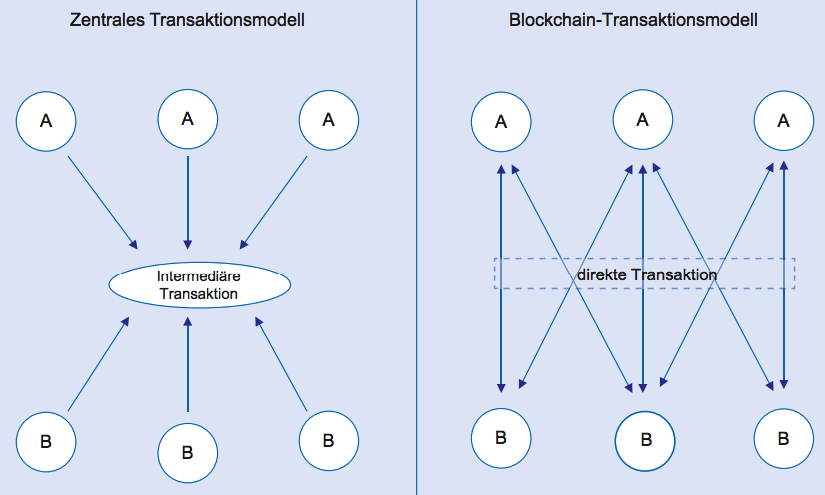
\includegraphics[width=1.0\linewidth]{pictures/change-in-transaction-model-blockchain}
	\caption[Transaktionsmodell Blockchain]{Transaktionsmodell Blockchain \textcolor{red}{QUELLE}}
	\label{fig:change-in-transaction-model-blockchain}
\end{figure}

Wird von einem der Teilnehmer eine Transaktion ausgelöst, wird diese nicht durch einen Intermediär sondern durch das Netzwerk erfasst und verarbeitet (Abbildung \ref{fig:change-in-transaction-model-blockchain}). Ein neuer \textit{Block} wird erschaffen und validiert wie es durch das Konsensprotokoll festgelegt wird. Dabei können solche \textit{Blockchain} Systeme unterschiedlich ausgeprägt sein. Dies zeigt sich zb. an der Art des Zugriffs, also wer darf Transaktionen lesen, wer darf sie schreiben. Außerdem kann der Mechanismus zur Konsensfindung je System anders sein.

% \citep{Abeyratne2016}
% \citep{Casino2019}

% \citep{Platzer2014}
% \citep{Narayanan2016}
% \citep{Burgwinkel2016}

% \citep{Gayvoronskaya2017}
% \citep{Vigna2017}
% \citep{JPMorgan2018}
% \citep{Buhl2017}
% \citep{Maull2017}
% \citep{Technik2018}
% \citep{Mitschele2018}
% \citep{Neugebauer2018}
% \citep{Min2018}


\subsubsection{Begriffliche Abgrenzung}

Die am häufigsten verwendeten Begriffe werden im Folgenden anhand eines Schichtenmodells (Abbildung \ref{fig:layer-model-blockchain}) erklärt und voneinander abgegrenzt. Jede Schicht wird in der Abbildung durch einen Balken dargestellt und ist unabhängig von den darüber liegenden Schichten. Von oben nach unten gelesen stehen die Schichten in einer \glqq ist enthalten in\grqq{} Beziehung zueinander. Entsprechend verlaufen die Schichten von einer konkreten Ausprägung zu einem abstrakten technologischen Konzept. Nachfolgend werden die einzelnen Schichten genauer erklärt.

\begin{figure}[H]
	\centering
	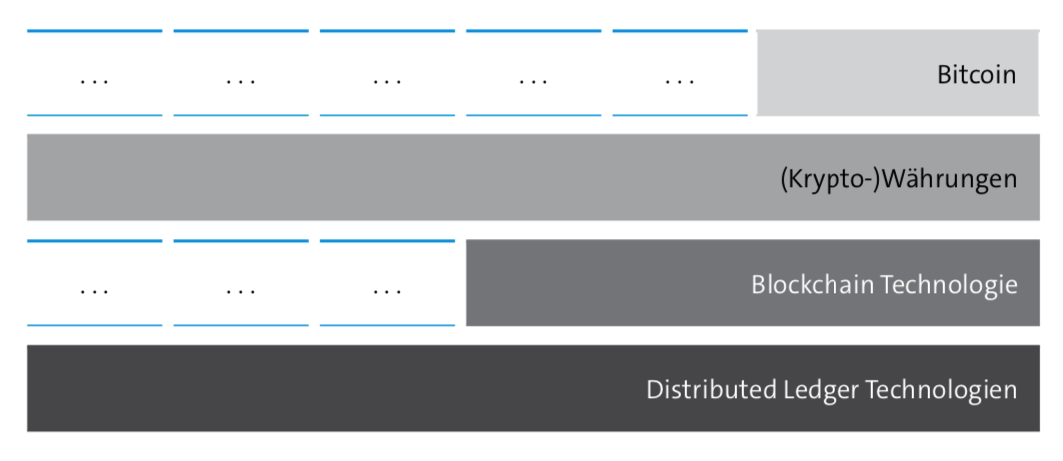
\includegraphics[width=1.0\linewidth]{pictures/layer-model-blockchain}
	\caption[Schichtenmodell \textit{Blockchain} Begriffe]{Schichtenmodell \textit{Blockchain} Begriffe \textcolor{red}{QUELLE}}
	\label{fig:layer-model-blockchain}
\end{figure}

\paragraph{Distributed Ledger}$~~$\\
Der \textit{Distributed Ledger} bildet die Basis des Schichtenmodells. Er ist im Grunde genommen ein klassisches Betandsbuch, das über einen Mechanismus verfügt, es auf alle teilnehmenden Parteien zu verteilen. \textit{Distributed Ledger} existieren bereits seit längerer Zeit und sind meist auf der technischen Basis einer verteilten Datenbank mit einer Logik auf Programm- oder Datenbankseite versehen, die aus der reinen Datenbank ein Bestandsbuch macht.

Distributed Ledger Technologie wird zunehmend synonym zum bisherigen Gebrauch von \textit{Blockchain} genutzt, um die Entwicklungen nach dem Bitcoin und den Kryptowährungen von eben diesen begrifflich abzugrenzen.

\paragraph{Blockchain-Technologie}$~~$\\
Die \textit{Blockchain} ist eine Form, einen \textit{Distributed Ledger} zu organisieren und zu implementieren. Auf die technische Implementierung der \textit{Blockchain} wird in den folgenden Kapiteln näher eingegangen; zur Begriffsbestimmung seien hier die grundlegenden Eigenschaften aufgezählt, die der \textit{Blockchain} in den letzten Jahren die steigende Aufmerksamkeit ermöglich haben:

\begin{itemize}
  \item Dezentralisiert
  \item Peer-to-Peer
  \item Transparenz und Anonymität
  \item Vertrauen
\end{itemize}

Blockchain gehört zu den bekanntesten Distributed-Ledger-Technologien. Aus diesem Grund wird die Bezeichnung Blockchain-Technologie in dieser Arbeit synonym für Distributed-Ledger-Technologien benutzt. Auf die technischen Eigenschaften von weiteren Ausprägungen der Distributed-Ledger-Technologien wird in dieser Arbeit daher nicht eingegangen.

\paragraph{Kryptowährungen}$~~$\\
Mit der \textit{Blockchain} als Basistechnologie lassen sich darauf aufbauende komplexe Systeme, wie z.B. Währungen abbilden. Wie in Kapitel \ref{blockchain-definition} erwähnt wurde die Blockchain-Technologie als erstes im Zusammenhang mit einer Kryptowährungen, dem Bitcoin, beschrieben. Die \textit{Blockchain} ist somit ein Nebenprodukt einer technischen Plattform, die eine kryptographische Währung erschuf und gleichzeitig ein System implementierte, um diese Währung zu nutzen und zu handeln.

Neben dem Bitcoin existiert eine Reihe weiterer Kryptowährungen, die sich zum Teil der dem Bitcoin zugrunde liegenden öffentlichen \textit{Blockchain} bedienen. Genannt seien hier z.B. Litecoin oder Dogecoin. Es existieren darüber hinaus Kryptowährungen, die eigene Blockchains zur Basis haben - zum Teil auf einer komplett eigenen technischen Implementierung. Vertreter hierfür sind z.B. Ethereum, Ripple oder Iota \citep[siehe auch][]{Buterin2014, carVertical, JPMorgan2018}.

\paragraph{Bitcoin}$~~$\\
Der Bitcoin ist die Kryptowährung, die auf der ursprünglichen \textit{Blockchain} gehandelt wird. Im Rahmen dieser Arbeit wird der Bitcoin und andere Kryptowährungen nicht weiter betrachtet.

\subsubsection{Arten von \textit{Blockchain}} \label{Arten-von-Blockchain}
Bei der Auswahl der Art einer \textit{Blockchain} trifft man auf zwei Widersprüche die nachfolgend kurz erläutert sind. Darauf folgt eine Betrachtung der Konfliktursachen und die sich daraus ableitenden Kategorien in die sich ein Blockchain System einordnen lässt.

\paragraph{Transparenz vs. Vertraulichkeit}$~~$\\
Verwendet man eine \textit{Blockchain} werden Besitzverhältnisse durch die Transaktionshistorie ermittelt. Dabei lässt sie eine \textit{Blockchain} mit einem öffentlichen Register vergleichen. Im Sinne der Übertragung von Eigentum sind Offenheit und Transparenz zwei wesentliche Eigenschaften der Blockchain. Durch diese Offenheit ist jeder Teilnehmer in der Lage alle Transaktionen einzusehen und auf Manipulationen zu prüfen.

Dieses Vorgehen steht im Gegensatz zur Vertraulichkeit, die in bestimmten Bereichen unabdingbar ist. Durch Vertraulichkeit werden Informationen wie die Transaktionsdaten oder deren Details (beteiligte Konten oder transferierte Menge) vor unbefugter Einsicht geschützt. Hierdurch entsteht der Widerspruch zwischen Transparenz auf der einen Seite und Anforderungen an die Vertraulichkeit auf der anderen Seite \citep{Drescher2017}.

\paragraph{Sicherheit vs. Geschwindigkeit}$~~$\\
Die Datenstruktur einer \textit{Blockchain} sichert die Transaktionshistorie vor Manipulationen und Fälschungen. Jeder neue \textit{Block} der in der \textit{Blockchain} gespeichert werden soll muss vom Netzwerk durch das Lösen einer kryptographischen Aufgabe erzeugt und der Datenstruktur hinzugefügt werden. Dadurch ist es ziemlich aufwendig die Transaktionshistorie nachträglich zu manipulieren oder zu fälschen. Durch diesen Sicherheitsmechanismus sinkt die Geschwindigkeit mit der ein \textit{Blockchain} Netzwerk neue Transaktionen verarbeiten kann. Moderne Applikationen erfordern Geschwindigkeit und Skalierbarkeit was im direkten Kontrast zum erwähnten Sicherheitskonzept einer \textit{Blockchain} steht \citep{Drescher2017}.

\paragraph{Ursachen der Konflikte}$~~$\\
Zwei grundlegende Operationen eines \textit{Blockchain} Netzwerks sind Ursache für die beiden beschriebenen Widersprüche - Schreiben und Lesen von Transaktionsdaten. Der Konflikt zwischen Transparenz und Vertraulichkeit ist auf die Lese-Operationen einer \textit{Blockchain} zurückzuführen. Je offener die Leseberechtigungen einer \textit{Blockchain} sind, desto höher ist die Transparenz und desto niedriger ist die Vertraulichkeit der Transaktionsdaten. Die Schreib-Operationen sind für den Widerspruch zwischen Sicherheit und Geschwindigkeit verantwortlich. Je restriktiver die Berechtigungen zum Schreiben innerhalb des \textit{Blockchain} Netzwerks sind, desto höher ist die Geschwindigkeit mit der Transaktionen verarbeitet werden können. In Tabelle \ref{tab:technical-restricts-blockchain} werden die technischen Beschränkungen, der Widerspruch und die Operation innerhalb der \textit{Blockchain} zusammengefasst \citep{Drescher2017}.

\begin{table}[H]
	\begin{tabular}{@{}lll@{}}
		\toprule
		\textbf{Beschränkung} & \textbf{Widerspruch}            & \textbf{Blockchain Operation} \\
		\midrule
		Keine Vertraulichkeit & Transparenz vs. Vertraulichkeit & Transaktionshistorie lesen    \\ \addlinespace
		Skalierbarkeit        & Sicherheit vs. Geschwindigkeit  & Transaktionen schreiben       \\
		\bottomrule
	\end{tabular}
	\caption{Technische Beschränkungen der \textit{Blockchain} und ihre Ursachen}
    \label{tab:technical-restricts-blockchain}
\end{table}

\paragraph{Public vs. Private}$~~$\\
Betrachtet man die Berechtigungen zum Lesen innerhalb eines \textit{Blockchain} Netzwerks in der einfachsten Form muss das System zwischen Transparenz und Vertraulichkeit entscheiden. Entweder es werden allen Teilnehmern Leseberechtigungen zugeteilt oder nur einer ausgewählten Gruppe von Teilnehmern. Anhand des Kriterium, welcher Teilnehmer im Netzwerk neue Transaktionen erstellen und die Historie lesen kann, lässt sich eine \textit{Blockchain} als öffentliche oder private \textit{Blockchain} charakterisieren \citep{Drescher2017}.

\paragraph{Permissioned vs. Permissionless}$~~$\\
Die Schreibrechte bestimmen für ein \textit{Blockchain} Netzwerk den Grad der Skalierbarkeit. Werden Schreibrechte in ihrer einfachsten Form zugeteilt und alle Teilnehmer sind berechtigt Schreib-Operationen auszuführen, erhöht sich der Arbeitsaufwand je Teilnehmer der zur Berechnung nötigt wird. Dies ist für die Sicherheit des Netzwerk positiv, wirkt sich aber negativ auf die Geschwindigkeit aus. Durch die Geschwindigkeit wird das Netzwerk in der Skalierbarkeit beschränkt. Teilt man hingegen nur einer Gruppe von Teilnehmern Schreibrechte zu, ist der Arbeitsaufwand im Vergleich niedrig. Hierdurch kann das Netzwerk Transaktionen vergleichsweise schnell verarbeiten und ist dadurch selbst skalierbarer \citep{Drescher2017}.

\begin{table}[H]
	\resizebox{\textwidth}{!}{%
	\begin{tabular}{@{}lll@{}}
	\toprule
								& \textbf{Permissionless}                                                                                                               & \textbf{Permissioned}                                                                                                                    \\
	\midrule
	\textbf{Public}             & \begin{tabular}[c]{@{}l@{}}Bitcoin, Ethereum, IOTA\\ \\ Jeder kann validieren\\ Jeder kann teilnehmen\end{tabular}                    & \begin{tabular}[c]{@{}l@{}}Ethereum 2.0\\ \\ Ausgewählte Gruppe kann validieren\\ Jeder kann teilnehmen\end{tabular}                     \\
	\midrule
	\textbf{Consortium/Private} & \begin{tabular}[c]{@{}l@{}}Interplanetary Database(IPDB)\\ \\ Jeder kann validieren\\ Ausgewählte Gruppe kann teilnehmen\end{tabular} & \begin{tabular}[c]{@{}l@{}}Hyperledger, Quorum\\ \\ Ausgewählte Gruppe kann validieren\\ Ausgewählte Gruppe kann teilnehmen\end{tabular} \\
	\bottomrule
	\end{tabular}%
	}
	\caption{Arten von Blockchain Netzwerken (eigene Darstellung)}
	\label{tab:types-of-blockchain-networks}
\end{table}

\noindent
Alle zuvor beschriebenen Eigenschaft einer Blockchain ermöglichen es eine Matrix mit zwei Dimensionen zu modellieren in die sich nahezu sämtliche Blockchain Lösungen einordnen lassen. Ausgenommen sind etwaige Mischformen, die für sehr spezielle Anwendungsfälle konzipiert wurden und sich beispielsweise aus einer Kombination einer öffentlichen und konsortialen Blockchain zusammensetzen. Tabelle \ref{tab:types-of-blockchain-networks} zeigt diese Matrix. Die vertikale Achse beschreibt in diesem Fall die Anonymität der Teilnehmer. Diese reicht von vollständiger Anonymität\footnote{Anonymität meint hier eine Pseudo-Anonymität, da aus technischer Sicht mit einigem Aufwand der Teilnehmen klar identifiziert werden kann.} bis zur Offenlegung und direkten Verknüpfung zwischen einem Teilnehmer des Netzwerks und einer Entität (Person, Maschine oder Unternehmen) in der realen Welt. Auf der horizontalen Achse wird das Vertrauen in die Validatoren abgebildet. Konkret können entweder alle Teilnehmer auch als Validatoren auftreten (Permissionless) oder es wird eine Gruppe von Teilnehmern zum validieren von Transaktionen gebildet, die definierte Anforderungen erfüllen (Permissioned). An den Schnittpunkten der Zeilen und Spalten wurden Beispiele für Implementationen der jeweiligen Kombination eingefügt.

%\subsubsection{Technologischer Hintegrund}
%Eine \textit{Blockchain} operiert auf einem \textit{Peer-to-Peer} Netzwerk in welchem jeder \textit{Knoten} eine exakte Kopie der Transaktionshistorie vorhält. Eine \textit{Blockchain} ist somit eine verteilte Datenbank, die eine kontinuierliche Liste von Transaktionen speichert und durch kryptographische Mechanismen vor Manipulation schützt. Transaktionen werden anhand eines Konsensusprotokolls validiert und zur Liste der Transaktionen hinzugefügt \citep{Nakamoto2009}.

\subsubsection{Peer-to-Peer Netzwerke}
Ein \textit{Peer-to-Peer} Netzwerk ist der Gegensatz zum klassischen \textit{Client-Server-Modell}, bei dem ein \textit{Server} einen Dienst zur Verfügung stellt und ein oder mehrere \textit{Clients} diesen Dienst abrufen und nutzen. Bei einem \textit{Peer-to-Peer} Netz sind alle Teilnehmer, die sog. \textit{Peers}, gleichberechtigt und können Dienste anbieten und auch konsumieren. \textit{Peer-to-Peer} Netzwerke operieren als \textit{Overlay-Netze}\footnote{Ein \textit{Overlay-Netz} baut auf ein bestehendes Netz (\textit{Underlay Netz}) auf. Es kann mit eigenen Protokollen arbeiten und selbst als \textit{Underlay Netz} fungieren.\citep{Andersen2001}} auf dem Internet. Einige der häufigsten Eigenschaften von \textit{Peer-to-Peer} Netzwerken sind nach \citet{Steinmetz2005}:

\begin{itemize}
  \item Heterogenität zwischen den \textit{Peers} in Bezug auf Bandbreite, Rechenkraft und Speichergröße
  \item Qualität einzelner \textit{Peers} in Form von Verfügbarkeit und Verbindungsstärke lässt sich nicht voraussetzen
  \item Client-Server-Funktionalität wird für \textit{Peers} ermöglicht, um Dienste und Ressourcen anzubieten und zu konsumieren
  \item Austausch von Diensten und Ressourcen unter allen \textit{Peers} gewährleistet
  \item Bereitstellung von Such-Funktionen durch ein zusätzliches \textit{Overlay-Netz}
  \item Autonomie der \textit{Peers} in punkto Ressourcenbereitstellung
  \item Das \textit{Peer-to-Peer} Netzwerk organisiert sich selbst und nicht durch Dritte
\end{itemize}

\subsubsection{Kryptografisches Hashing}
Kryptografisches Hashing gehört zu einem der wichtigsten Instrumente der Kryptografie und bildet einen eigenen Teilbereich der Kryptografie. Mit einer kryptografischen Hash-Funktion lässt sich aus einem beliebig langen Wort (oder Datensatz) eine Zeichenkette mit fixer Stellenanzahl generieren. Die jeweilige Ausgabelänge wird in Bit angegeben. Formal ist eine Hash-Funktion definiert als

\begin{equation}
	f:\left \{ 0,1 \right \}^{*} \mapsto \left \{ 0,1 \right \}^{n}
\end{equation}

Das Ergebnis wird als digitaler Fingerabdruck bezeichnet. Die Generierung des Hash-Werts ist nicht zwingend kryptografisch, denn nicht jede Hash-Funktion erfüllt alle Anforderungen einer kryptografischen Hash-Funktion \citep{Menezes1997, Diffie1976}. Dabei gilt, eine kryptografische Hash-Funktion muss folgende Kriterien erfüllen:

\begin{itemize}
	\item Eindeutigkeit
	\item Reversibilität
	\item Kollisionsresistenz
\end{itemize}

Mit der Eindeutigkeit ist gegeben, dass ein bestimmter Eingabewert immer zum selben Ausgabewert führt. Reversibilität beschreibt die Eigenschaft einer Hash-Funktion, das der Ausgabewert nicht in den ursprünglichen Eingabewert zurückberechnet werden kann. Die Kollisionsresistenz sorgt dafür, dass zwei unterschiedliche Eingabewerte nicht den gleichen Ausgabewert erzeugen. Abbildung \ref{fig:schema-hash-function} zeigt schematisch die Funktionsweise einer kryptografischen Hash-Funktion. Der Eingabewert, hier Urbild, wird durch die kryptografische Hash-Funktion in einen Ausgabewert (Hash-Wert) fester Länge transformiert.

\begin{figure}[H]
	\centering
	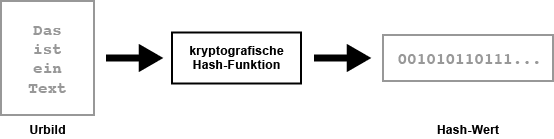
\includegraphics[width=1.0\linewidth]{pictures/schema-hash-function}
	\caption[Funktionsweise einer kryptografischen Hash-Funktion]{Funktionsweise einer kryptografischen Hash-Funktion \textcolor{red}{QUELLE Elektronik Kompendium}}
	\label{fig:schema-hash-function}
\end{figure}

\subsubsection{Signierte Transaktionen durch Public-Key-Infrastruktur}
Wird eine Transaktion von einem Teilnehmer erstellt und soll durch das Netzwerk validiert werden kommen digitale Signaturen zum Einsatz. Digitale Signaturen gehören zur asymmetrischen Kryptographie und werden dazu verwendet die Urheberschaft und Integrität einer Nachricht oder, im Falle der Blockchain, einer Transaktion zu prüfen.\citep{Beutelspacher2010, Menezes1997}

\begin{figure}[H]
	\centering
	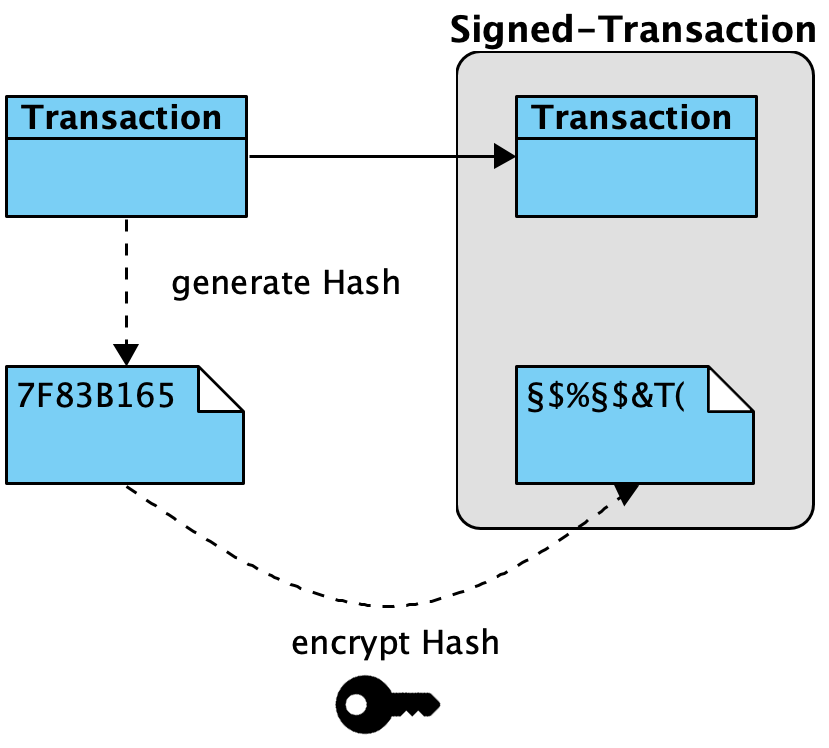
\includegraphics[width=0.7\linewidth]{pictures/digital-signatures-create}
	\caption[Erstellen einer digitalen Signatur]{Schematische Darstellung für das Erstellen einer digitalen Signatur (in Anlehnung an \citet{Drescher2017})}
	\label{fig:digital-signatures-create}
\end{figure}

In Abbildung \ref{fig:digital-signatures-create} wird das digitale Signieren einer Transaktion verdeutlicht. Der Prozess startet oben links in der Abbildung mit einer Transaktion. Durch Anwendung einer kryptographischen Hashfunktion wird ein Hash gebildet. Dieser Hashwert wird anschließend mit dem privaten Schlüssel des Erstellers verschlüsselt. Dieser verschlüsselte Hashwert ist die digitale Signatur und zusammen mit der Transaktion bilden sie die digital signierte Transaktion. Durch die Verwendung der \ac{pki} ist die digitale Signatur auf zwei Arten einzigartig. Zum einen kann der Ersteller der Signatur eindeutig zugeordnet werden und zum anderen wird die Integrität der Transaktion sichergestellt \citep{Drescher2017}.

\begin{figure}[H]
	\centering
	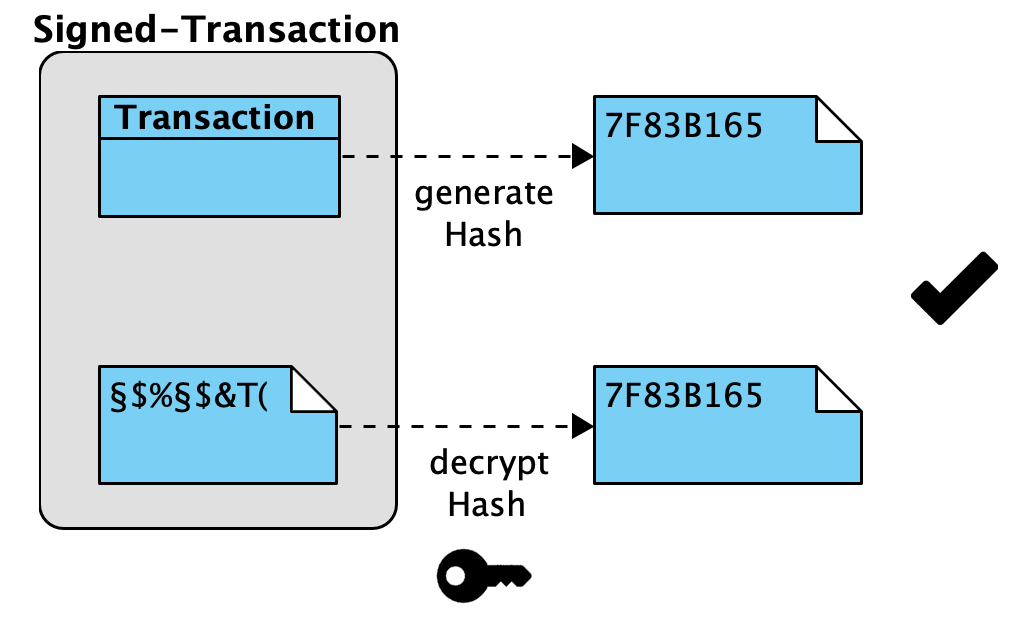
\includegraphics[width=0.7\linewidth]{pictures/digital-signatures-validate-positive}
	\caption[Prüfen einer digitalen Signatur]{Erfolgreiche Prüfung einer digitalen Signatur (in Anlehnung an \citet{Drescher2017})}
	\label{fig:digital-signatures-validate-positive}
\end{figure}

Soll eine signierte Transaktion vom Netzwerk verarbeitet und erfolgreich verbucht werden müssen zwei Eigenschaften erfüllt sein. Die Urheberschaft muss eindeutig zuzuordnen sein und die Integrität der Transaktion darf nicht verletzt worden sein. Dazu wird wie in Abbildung \ref{fig:digital-signatures-validate-positive} zuerst mit dem öffentlichen Schlüssel des Absenders die digitale Signatur entschlüsselt. Gelingt dies, ist sichergestellt das der Ersteller der digitalen Signatur eindeutig über die \ac{pki} zugeordnet werden kann. Im zweiten Schritt wird aus der Transaktion der Hashwert gebildet und mit der entschlüsselten digitalen Signatur verglichen. Sind beide Werte gleich ist garantiert, dass die Transaktion auf dem Weg der Übermittlung nicht manipuliert wurde \citep{Drescher2017}.

Stellt sich bei der Überprüfung der signierten Transaktion heraus, dass die Hashwerte nicht übereinstimmen können zwei Gründe dafür verantwortlich sein. Entweder wurde die eigentliche Transaktion während der Übermittlung von einem Angreifer manipuliert oder die Transaktion wurde nicht vom vermeintlichen Teilnehmer des Netzwerks autorisiert \citep{Drescher2017}. Abbildung \ref{fig:digital-signatures-validate-negative} zeigt schematisch diese Situation.

\begin{figure}[H]
	\centering
	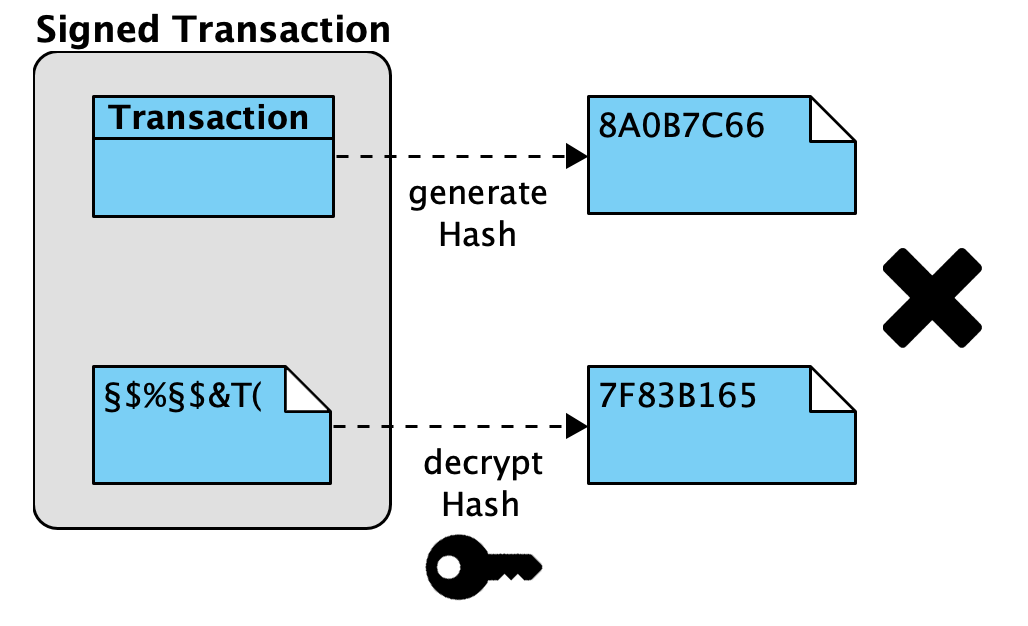
\includegraphics[width=0.8\linewidth]{pictures/digital-signatures-validate-negative}
	\caption[Manipulationerkennung durch digitale Signaturen]{Erkennung von Manipulation anhand der digitalen Signatur (in Anlehnung an \citet{Drescher2017})}
	\label{fig:digital-signatures-validate-negative}
\end{figure}

\subsubsection{Konsensmechanismen}
Es gibt hauptsächlich zwei Kategorien von Konsensmechanismen:

\begin{itemize}
	\item Lotterie-basiert
	\item Byzantinische Fehlervereinbarung
\end{itemize}

Die erste Kategorie wird auch Nakamoto-Konsens genannt nach dem Pseudonym des Bitcoin Erfinders Satoshi Nakamoto. Der Konsensmechanismus wählt den Prüfer, d.h. den Knoten, der entscheidet, welcher der nächste Block ist, der an die Blockchain angehangen wird. Dabei ist die Wahl eine Lotterieziehung. Der Gewinner ist der Validierer. Jeder neue Block erfordert auch eine neue Ziehung eines Validierers. Die Auswahl durch eine Lotterie reduziert die Wahrscheinlichkeit, dass ein kompromittierter Knoten einen gefälschten Block validiert. Hierbei folgt die Lotterie keiner gleichwertigen Verteilung. Jeder Mechanismus definiert seine eigene Wahrscheinlichkeitsverteilung anhand eine bestimmte Eigenschaft des Gewinners bevorzugt wird. So besitzt jeder Lotterie-basierte Konsensmechanismus ein anderes Vertrauensmodell. Bitcoin beispielsweise verwendet den bekanntesten Mechanismus - \acf{pow}. Daneben gibt es wie beschrieben noch einige andere Mechanismen wie \acf{pos}, \acf{posp} oder \acf{poet}.

\acf{bft}-Systeme bilden die Basis für Mechanismen der zweiten Kategorie. \ac{bft}-Systeme sind so konzipiert, dass sie auch bei Ausfall einiger Teilnehmer des Netzwerks weiterhin funktionieren. Dabei kann der Ausfall unfreiwillig (z.B. ein teilnehmender Knoten ist außer Betrieb) oder freiwillig (z.B. ein Angreifer kontrolliert den fehlerhaften Knoten) sein. \ac{bft}-Systeme verwenden Abstimmungsmechanismen, um einen Konsens herstellen zu können. Der verwendete Mechanismus legt das Vertrauensmodell fest. Der \acf{pbft} Mechanismus ist der bekannteste Mechanismus dieser Kategorie.
Außerdem sind hybride Konsensmechanismen möglich die eine Mischung aus Lotterie und \ac{bft} darstellen. Nachfolgend sollen die beiden meist verwendeten Konsensmechanismen kurz erläutert werden.

\paragraph{Proof-of-Work}$~~$\\
Das Konzept des \acf{pow} existierte schon vor der ersten Blockchain Applikation (Bitcoin). Die erste moderne Anwendung wurde 1996 von Adam Back unter dem Namen \glqq Hashcash\grqq{} eingereicht. Diese Anwendung hat auf Grundlage des SHA265-Algorithmus einen \ac{pow} Mechanismus eingesetzt um E-Mail Spam zu verhindern \citep{Back2002}.

Der Mechanismus des \ac{pow} kann relativ simpel beschrieben werden. Es ist die Tatsache, dass ein Teilnehmer des Netzwerks allen anderen Teilnehmern das Ergebnis der von ihm durchgeführten Berechnungen vorlegt. Die durchzuführenden Operationen sind an sich nicht kompliziert, allerdings müssen sie so oft durchgeführt werden, dass der Teilnemer eine erhebliche Rechenleistung dafür aufbringen muss. Daher spricht man von \glqq Proof-of-Work\grqq{}, da der Teilnehmer mit einem korrekten Ergebnis einen Nachweis seiner geleisteten Arbeit gibt. Konkret muss der Teilnehmer ein Ergebnis finden, das mit einer  bestimmten Anzahl an führenden Nullen beginnt. Je größer die Anzahl der führenden Nullen ist, desto schwierieger ist es für den Teilnehmer ein valides Ergebnis zu finden. Die Anzahl der Nullen bzw. die Schwierigkeit wird an die Anzahl der Teilnehmer und ihrer Rechenleistung im Netzwerk angepasst, sodass ein neues Ergebnis in festen Intervallen gefunden werden kann.\footnote{Im Bitcoin Blockchain Netzwerk wird die Schwierigkeit dauerhaft so angepasst, dass nur alle 10 Minuten ein neuer Block berechnet werden kann.} Für die Berechnung des Ergebnisses fügt der Teilnehmer zu den eigentlichen Transaktionsdaten eine sogenannte \glqq Nonce\grqq{} hinzu. Aus diesen Daten versucht der Teilnehmer das Ergebnis zu berechnen mit der entsprechenden Anzahl an führenden Nullen. Bei jeder Runde wird die \glqq Nonce\grqq{} verändert. Dies wird solange durchgeführt bist das Ergebnis zur aktuellen Schwierigkeit im Netzwerk passt.

\paragraph{Practical Byzantine Fault Tolerance}$~~$\\
Das \ac{pbft}-Modell konzentriert sich in erster Linie auf die Bereitstellung einer Zustandsmaschine, die byzantinische Fehler (kompromittierte Knoten oder Netzwerkteilnehmer) toleriert. Dies geschiet durch die Annahme, dass es unabhängige Knotenausfälle und manipulierte Nachrichten gibt. Der Algorithmus wurde für den Einsatz in asynchronen Systemen konzipiert und optimiert auf hohe Performance. Im Wesentlichen sind alle Knoten im \ac{pbft}-Modell in Reihe angeordnet, wobei ein Knoten als Primärknoten und die restlichen Knoten als Backupknoten bezeichnet werden. Alle Knoten innerhalb des Systems kommunizieren untereinander mit dem Ziel einen einheitlichen Zustand des Systems zu finden. Die Knoten müssen dabei nachweisen, das eine Nachricht von ihnen stammt und das diese Nachricht während der Übertragung nicht manipuliert wurde \citep{Tuan2017}.

Damit das \ac{pbft}-Modell funktioniert, wird davon ausgegangen, dass die Anzahl der kompromittierten Knoten im Netzwerk nicht größer oder gleich \nicefrac{1}{3} der Gesamtanzahl an Knoten im Netzwerk ist. Je mehr Knoten das Netzwerk bilden, desto mathematisch unwahrscheinlicher ist es, dass eine Anzahl von Knoten die sich \nicefrac{1}{3} der Gesamtknotenanzahl nähert kompromittiert ist.

Jede Runde des \ac{pbft}-Konsens, genannt \textit{Views}, besteht aus 4 Phasen. Das Modell folgt dabei eher dem Format \glqq Kommandant und Offiziere\grqq{} durch die Anwesenheit des Primärknotens. Beim byzantinischen Generalsproblem sind alle Generäle gleichwertig, was hier nicht der Fall ist. Die Phasen des \ac{pbft}-Konsens sehen wie folgt aus.

\begin{enumerate}
	\item Ein Client sendet eine Anfrage an den Primärknoten, um eine Serviceoperation durchzuführen.
	\item Der Primärknoten sendet die Anfrage an alle Backupknoten.
	\item Die Knoten führen die Anfrage aus und senden eine Antwort an den Client.
	\item Der Client erwartet \(3f + 1\) Antworten von verschiedenen Knoten mit dem gleichen Ergebnis.\footnote{Mit \(f\) ist die Anzahl an tollerierbaren kompromittierten Knoten gemeint.} Das Ergebnis ist das Ergebnis der Serviceoperation.
\end{enumerate}

Alle Knoten müssen die Anforderung erfüllen deterministisch zu operieren und im gleichen Zustand mit der Operation zu beginnen. Das Endergebnis ist, das sich alle nicht-kompromittierten Knoten auf die Reihenfolge der Datensätze einigen und dies geschlossen akzeptieren oder ablehnen.

Der Primärknoten wird in jeder \textit{View} nach dem Round-Robin Verfahren ausgewählt und kann auch ausgetauscht wurde durch eine Erweiterung des Modells. Ein Austausch kann durchgeführt werden, wenn der Primärknoten die Anfrage nicht innerhalb eines bestimmten Zeitlimits an die Backupknoten weiterleitet.

\textcolor{red}{Quellen ergänzen!}
